\graphicspath{ {Chapters/images/} }
\chapter{Result And Discussion}

We test accuracy and detection power of our method called SemiAssembler in comparison with MindTheGap using a variety of simulations and real sequencing data. MindTheGap is specific for the detection and assembly of insertions, and thus only insertions can be compared with MindTheGap.   
The simulation data sets used Escherichia coli K12 as the reference genome, whereas paired-end reads (insert size 450bp) and mate pair reads (insert size 4.5kb) are randomly sheared by wgsim. Real sequencing data sets are from two rice species (called TN67 and Shio),and $O. Sativa$ is used as the reference genome. Paired-end (with insert size 400bp) and mate-pair (with insert size 3kb) libraries were constructed and sequenced. These paired-end and mate-pair reads were separately aligned onto the reference genome using BWA-aln to produce standard SAM alignments, which are the input of our method. Paired-end reads and reference genome sequence are the input of MindTheGap. Table 4.1 shows the information of simulated data and real sequencing data. 

\begin{table}[!ht]
    \centering
    \begin{tabular}[t]{l|c|c|c|}
      & Simulated data set & Real data set & Real data set  \\
      \hline
      Species & {E.coli} & {TN67} & {Shio} \\
      Reference & E.coli &  \multicolumn{2}{|c|}{O. Sativa} \\     
      \cline{3-4}
      Genome Size & 4,641,653 bp &  \multicolumn{2}{|c|}{373,245,519 bp} \\
      \cline{3-4}
      Coverage of Paired-end & 25x & 33x & 33x \\
      Insert size of Paired-end & 450 & 450 & 450 \\
      Coverage of Mate-pair & 25x & 106x & 108x \\
      Insert size of Mate-pair & 4500 & 3672 & 4001 \\
      Number of Insertions & 30 & 6 & 3 \\ 
      Number of Deletions & 30 & 5 & 9 \\ 

      
   \end{tabular}
    \caption{}
    \label{}
\end{table}


\section{Results On Simulated Data Sets}


In order to understand the accuracy and power of our method  with respect to different sizes of insertions and deletions, we carried out several simulations at 25x coverage for each experiment. Only insertions will be compared with MindTheGap, which does not identify deletions.  

We simulate 30 insertions for each experiment. Figure 4.1 and Figure 4.2 illustrate the results of simulations with different sizes of insertions at 25x coverage. The detection power of SemiAssembler is less than that of MindTheGap, while both methods achieve the same precision. In terms of the assembled insertion sequences (Figure 4.4), the insertions assembled by our method is more accurate than that of MindTheGap. 
In terms of deletions, we also simulate 30 deletions for each experiment. Figure 4.5 illustrate the results of simulations with different sizes of deletions at 25x coverage. Even though we can not detect all insertions, SemiAssembler is still able to find most of the insertions ($>80$\%) with high accuracy.



\begin{figure}[ht]
\begin{center}
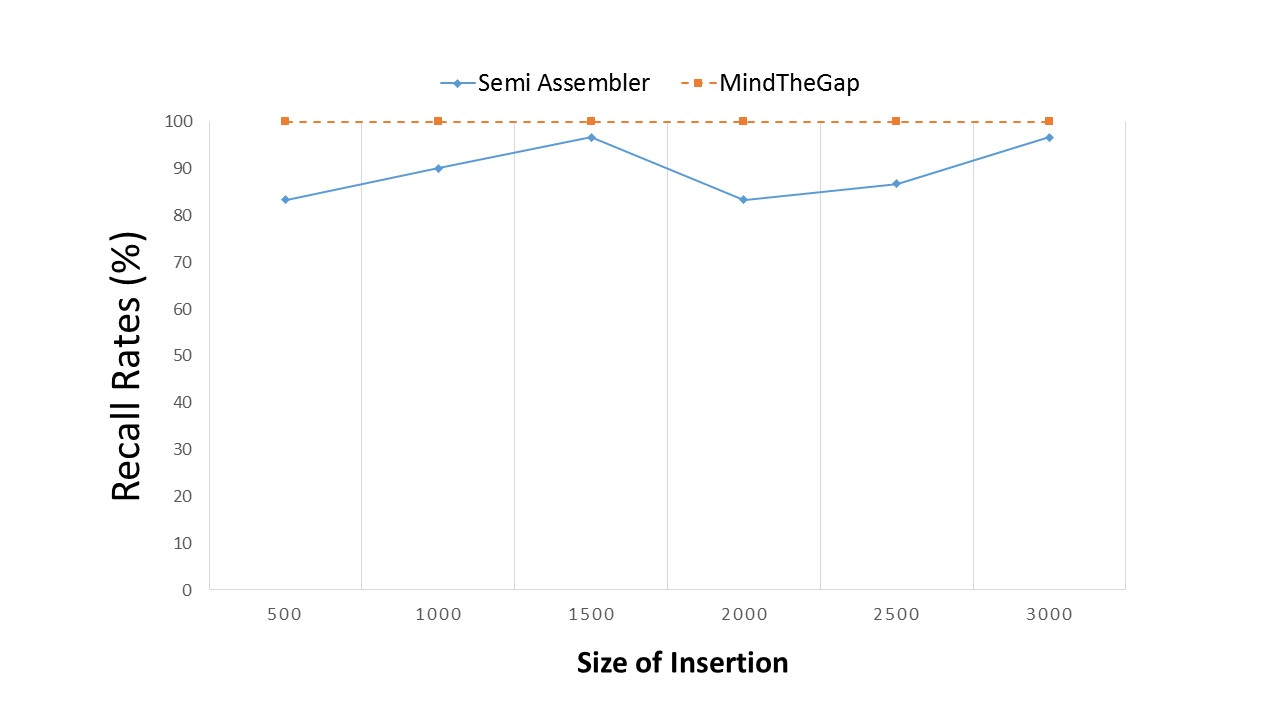
\includegraphics[scale=0.4]{r_recall2}
\caption{Recall rates of detecting insertions with different sizes. SemiAssembler can detect the insertions with high recall rates ($>80$\%).}
\label{}
\end{center}
\end{figure}

\begin{figure}[ht]
\begin{center}
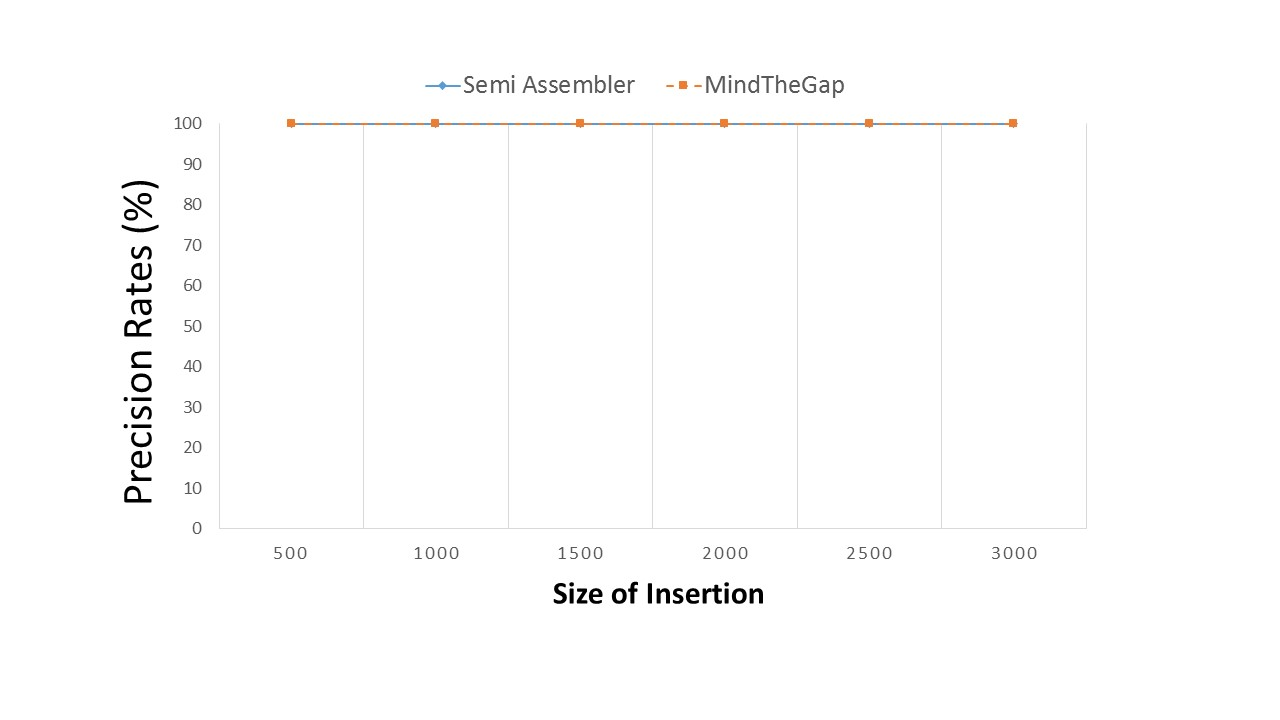
\includegraphics[scale=0.4]{r_prec}
\caption{Precision rates of detecting insertions with different sizes.}
\label{}
\end{center}
\end{figure}

\begin{figure}[ht]
\begin{center}
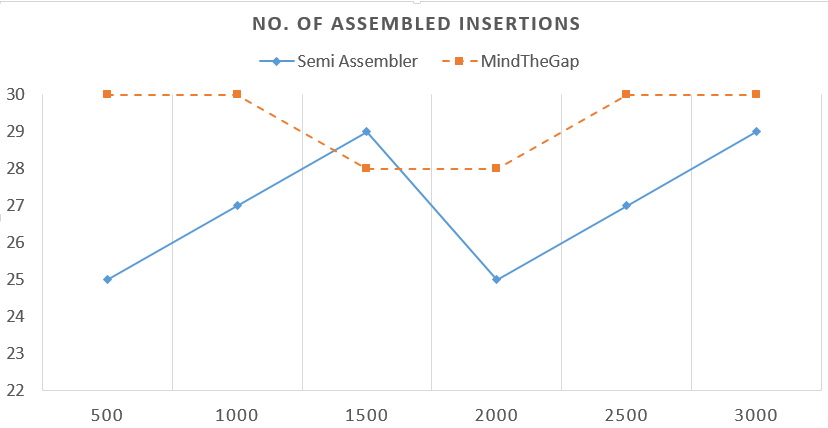
\includegraphics[scale=0.5]{r_assemble}
\caption{Number of assembled insertions.}
\label{}
\end{center}
\end{figure}

\begin{figure}[ht]
\begin{center}
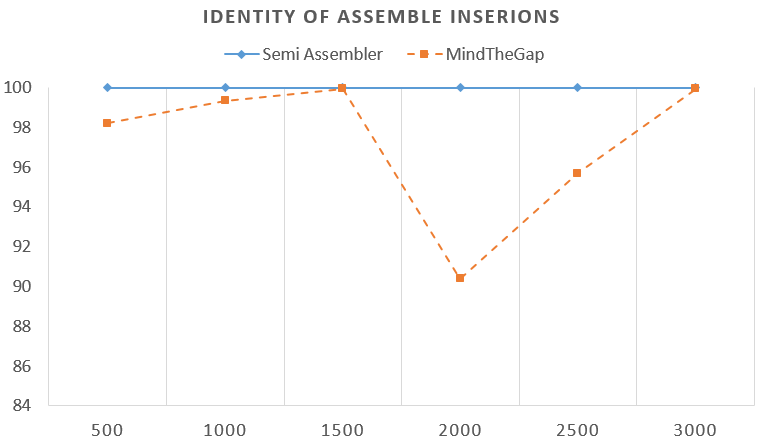
\includegraphics[scale=0.5]{r_id}
\caption{Identity of assembled insertions. SemiAssembler can assemble insertions with higher identities.}
\label{}
\end{center}
\end{figure}

\begin{figure}[ht]
\begin{center}
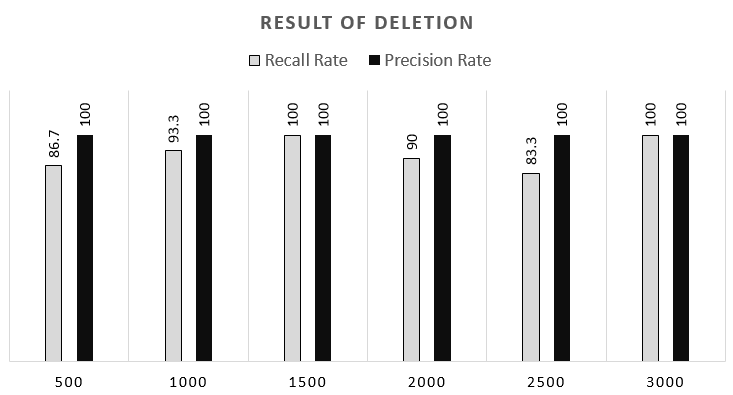
\includegraphics[scale=0.5]{deletion_result}
\caption{Simulated deletions of different sizes. SemiAssembler can detect the deletions ($>80$\%) with high accuracy.}
\label{}
\end{center}
\end{figure}




\clearpage


\section{Results On Real Sequencing Data Set}
We use real sequencing data sets of two rice species (called TN67 and Shio) to evaluate SemiAssembler. Sequencing data of TN67 and Shio are two related species derived from $O. Sativa$, in which the reference genome can be downloaded from the MSU rice genome annotation project. 

\subsection{Results of Detection of Large-sized Insertions}
We totally detect 403 insertions in TN67, and 273 insertions can be assembled. In Shio, we totally detect 190 insertions and assemble 127 insertions. We also run MindTheGap using the same data sets and compare the results with our method. MindTheGap totally detect 27344 insertions in TN67, and 5046 insertions can be assembled. In Shio, MindTheGap totally detect 23148 insertions, and 3582 insertions can be assembled. The total number of detected insertions with running MindTheGap is larger than our method because MindTheGap can detect small indels and our method detect large-sized insertions in this stage. Although we can not detect small insertions in this stage, we reflect small insertions/deletions and SNPs in the final stage of our method by using assembled contigs. 

In order to understand the accuracy and power of SemiAssembler, we use several validated large-sized insertions. Six insertions in TN67 and three insertions in Shio are detected by our method and validated by PCR and Sanger sequenced. Table 4.2 lists the number of detected and assembled insertions of both methods for TN67 and Shio.  In our mehod, we can detect all the nine insertions and assemble seven of them. On the other hand, MindTheGap can only detect seven insertions and assemble four of them. Most of these insertion sequences are composed of complex repeats difficult to be assembled. 



\subsection{Results of Detection of Large-sized Deletions}
In terms of deletions, we totally detect 422 deletions in TN67 and 353 deletions in Shio. We also use validated deletions to understand the accuracy and power of SemiAssembler. Three large-size deletions in TN67 and eight large-size deletions in Shio were validated by PCR and Sanger sequencing. We can detect 2 deletions in TN67 and 7 deletions in Shio. The two undetected deletions are due to the number of breakpoint reads is less than the default threshold (default 3). Table 4.2 list the results of detection of deletions for TN67 and Shio.


\begin{table}[!ht]
    \centering
    \begin{tabular}[t]{l|llll|ll}
   Species  & Method & No. of  & TP & Assembled  &  No. of & TP\\
             &        &Insertions    & &Insertions  & Deletions & \\
      \hline
      
     TN67 & SemiAssembler & 6 & 6 & 5 & 3 & 2\\
     TN67  & MindTheGap & 6 & 4 & 2 & - & -\\
     Shio & SemiAssembler & 3 & 3 & 2 & 8 & 7\\
     Shio  & MindTheGap & 3 & 3 & 2 & - & -\\

      
   \end{tabular}
    \caption{The number of validated insertions is in the column 'No. of Insertions'. The number of validated deletions is in the column 'No. of Deletions'.}
    \label{}
\end{table}



\subsection{Results of Detection of Indels}

Because the number of small indels is relatively large, the Sanger sequencing were not conducted and the exact sizes of these indels are not known. Nevertheless, as gel electrophoresis can separate DNA fragments based on their sizes, we can still compare the relative indel sizes between TN67 and Shio with those predicted by our method. For instance (see Figure 4.6), the indel at this locus of TN67 is larger than that of Shio.

\begin{figure}[ht]
\begin{center}
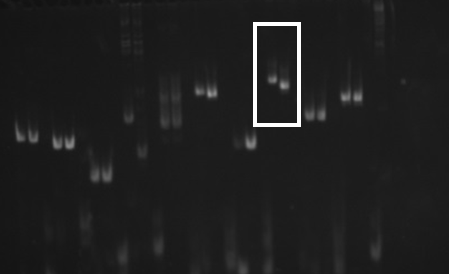
\includegraphics[scale=0.5]{ssr_screen}
\caption{Larger molecules move more slowly through the gel while the smaller molecules move faster. TN67 is on the left,and Shio is on the right in this gel electrophoresis.}
\label{}
\end{center}
\end{figure}

The major advantage of SemiAssembler is the assembled genome which is able to reflect small SNPs and indels across different species. Therefore, a subset of commonly-used biomarkers (from http://archive.gramen\-e.org/markers/microsat/) were screened using PCR in the TN67 and Shio genomes. 
These 75 biomarkers represent small indels ranging approximately from 1bp to 18bp. The gel electrophoresis shows that 42 of them may have indels between TN67 and Shio. In our method, we can recover 12 small insertions and 10 small deletions from these 42 small indel regions. On the other hand, MindTheGap can only detect one insertion from these 42 indels, and the only one detected insertion failed to be assembled. Table 4.4 list the results of detection of indels for TN67 and Shio.

\hfill
\begin{table}[!ht]
    \centering
    \begin{tabular}[t]{l|llll}
     Species & Method &  No. of Indels & Insertion & Deletion\\\\
      \hline
      
    TN67 & SemiAssembler & 12 & 8 & 4 \\
    TN67 & MindTheGap & 1 & 1 & - \\
    Shio & SemiAssembler & 10 & 1 & 9 \\
    Shio & MindTheGap & 0 & 0 & - \\\\
      
   \end{tabular}
    \caption{The result of recovering small indels in 42 validated small indels. The number of detected indels is in the column 'N'.}
    \label{}
\end{table}



